\documentclass[14pt]{extbook}
\usepackage{multicol, enumerate, enumitem, hyperref, color, soul, setspace, parskip, fancyhdr} %General Packages
\usepackage{amssymb, amsthm, amsmath, latexsym, units, mathtools} %Math Packages
\everymath{\displaystyle} %All math in Display Style
% Packages with additional options
\usepackage[headsep=0.5cm,headheight=12pt, left=1 in,right= 1 in,top= 1 in,bottom= 1 in]{geometry}
\usepackage[usenames,dvipsnames]{xcolor}
\usepackage{dashrule}  % Package to use the command below to create lines between items
\newcommand{\litem}[1]{\item#1\hspace*{-1cm}\rule{\textwidth}{0.4pt}}
\pagestyle{fancy}
\lhead{Makeup Progress Quiz 2}
\chead{}
\rhead{Version C}
\lfoot{5763-3522}
\cfoot{}
\rfoot{Spring 2021}
\begin{document}

\begin{enumerate}
\litem{
Construct the lowest-degree polynomial given the zeros below. Then, choose the intervals that contain the coefficients of the polynomial in the form $ax^3+bx^2+cx+d$.\[ \frac{-2}{5}, 3, \text{ and } \frac{7}{4} \]\begin{enumerate}[label=\Alph*.]
\item \( a \in [19, 21], b \in [7, 23], c \in [-120, -111], \text{ and } d \in [34, 44] \)
\item \( a \in [19, 21], b \in [-89, -86], c \in [61, 71], \text{ and } d \in [34, 44] \)
\item \( a \in [19, 21], b \in [87, 90], c \in [61, 71], \text{ and } d \in [-46, -36] \)
\item \( a \in [19, 21], b \in [-89, -86], c \in [61, 71], \text{ and } d \in [-46, -36] \)
\item \( a \in [19, 21], b \in [-104, -101], c \in [136, 145], \text{ and } d \in [-46, -36] \)

\end{enumerate} }
\litem{
Construct the lowest-degree polynomial given the zeros below. Then, choose the intervals that contain the coefficients of the polynomial in the form $x^3+bx^2+cx+d$.\[ 4 - 4 i \text{ and } 1 \]\begin{enumerate}[label=\Alph*.]
\item \( b \in [9, 11], c \in [39, 42], \text{ and } d \in [29, 35] \)
\item \( b \in [1, 6], c \in [-8, -1], \text{ and } d \in [0, 5] \)
\item \( b \in [1, 6], c \in [3, 11], \text{ and } d \in [-4, 3] \)
\item \( b \in [-12, -6], c \in [39, 42], \text{ and } d \in [-35, -30] \)
\item \( \text{None of the above.} \)

\end{enumerate} }
\litem{
Which of the following equations \textit{could} be of the graph presented below?
\begin{center}
    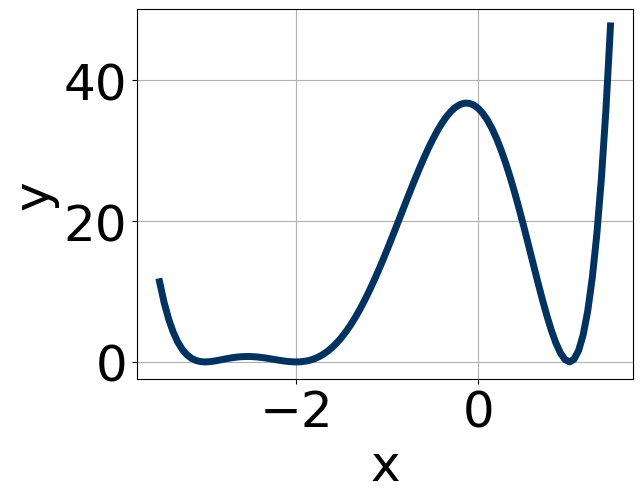
\includegraphics[width=0.5\textwidth]{../Figures/polyGraphToFunctionC.png}
\end{center}
\begin{enumerate}[label=\Alph*.]
\item \( 6(x + 2)^{8} (x - 1)^{6} (x + 3)^{10} \)
\item \( 2(x + 2)^{10} (x - 1)^{4} (x + 3)^{5} \)
\item \( 16(x + 2)^{8} (x - 1)^{9} (x + 3)^{7} \)
\item \( -12(x + 2)^{6} (x - 1)^{6} (x + 3)^{6} \)
\item \( -12(x + 2)^{10} (x - 1)^{10} (x + 3)^{11} \)

\end{enumerate} }
\litem{
Describe the zero behavior of the zero $x = -6$ of the polynomial below.\[ f(x) = 5(x - 8)^{9}(x + 8)^{6}(x - 6)^{14}(x + 6)^{9} \]\begin{enumerate}[label=\Alph*.]
\begin{multicols}{2}\item 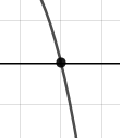
\includegraphics[width = 0.3\textwidth]{../Figures/polyZeroBehaviorCopyAC.png}\item 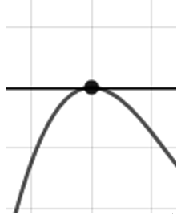
\includegraphics[width = 0.3\textwidth]{../Figures/polyZeroBehaviorCopyBC.png}\item 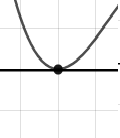
\includegraphics[width = 0.3\textwidth]{../Figures/polyZeroBehaviorCopyCC.png}\item 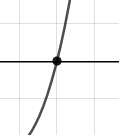
\includegraphics[width = 0.3\textwidth]{../Figures/polyZeroBehaviorCopyDC.png}\end{multicols}\item None of the above.
\end{enumerate} }
\litem{
Describe the zero behavior of the zero $x = 2$ of the polynomial below.\[ f(x) = 3(x - 2)^{3}(x + 2)^{8}(x + 5)^{6}(x - 5)^{7} \]\begin{enumerate}[label=\Alph*.]
\begin{multicols}{2}\item 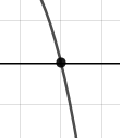
\includegraphics[width = 0.3\textwidth]{../Figures/polyZeroBehaviorAC.png}\item 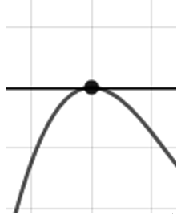
\includegraphics[width = 0.3\textwidth]{../Figures/polyZeroBehaviorBC.png}\item 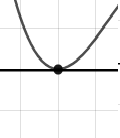
\includegraphics[width = 0.3\textwidth]{../Figures/polyZeroBehaviorCC.png}\item 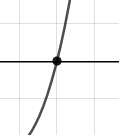
\includegraphics[width = 0.3\textwidth]{../Figures/polyZeroBehaviorDC.png}\end{multicols}\item None of the above.
\end{enumerate} }
\litem{
Construct the lowest-degree polynomial given the zeros below. Then, choose the intervals that contain the coefficients of the polynomial in the form $x^3+bx^2+cx+d$.\[ 5 + 3 i \text{ and } 1 \]\begin{enumerate}[label=\Alph*.]
\item \( b \in [7, 14], c \in [43.1, 45.1], \text{ and } d \in [32.85, 34.42] \)
\item \( b \in [-4, 2], c \in [-6.2, -5.8], \text{ and } d \in [4.36, 5.61] \)
\item \( b \in [-4, 2], c \in [-4.9, -1.2], \text{ and } d \in [1.56, 3.56] \)
\item \( b \in [-13, -2], c \in [43.1, 45.1], \text{ and } d \in [-35.09, -33.44] \)
\item \( \text{None of the above.} \)

\end{enumerate} }
\litem{
Construct the lowest-degree polynomial given the zeros below. Then, choose the intervals that contain the coefficients of the polynomial in the form $ax^3+bx^2+cx+d$.\[ \frac{2}{3}, \frac{-3}{2}, \text{ and } \frac{-5}{3} \]\begin{enumerate}[label=\Alph*.]
\item \( a \in [18, 20], b \in [44, 49], c \in [4, 9], \text{ and } d \in [-33, -23] \)
\item \( a \in [18, 20], b \in [10, 22], c \in [-45, -37], \text{ and } d \in [-33, -23] \)
\item \( a \in [18, 20], b \in [44, 49], c \in [4, 9], \text{ and } d \in [22, 35] \)
\item \( a \in [18, 20], b \in [-52, -44], c \in [4, 9], \text{ and } d \in [22, 35] \)
\item \( a \in [18, 20], b \in [69, 80], c \in [79, 85], \text{ and } d \in [22, 35] \)

\end{enumerate} }
\litem{
Describe the end behavior of the polynomial below.\[ f(x) = 7(x - 2)^{4}(x + 2)^{7}(x + 7)^{4}(x - 7)^{4} \]\begin{enumerate}[label=\Alph*.]
\begin{multicols}{2}\item 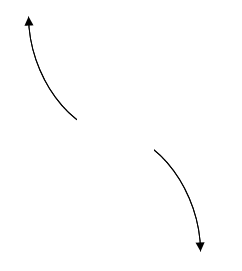
\includegraphics[width = 0.3\textwidth]{../Figures/polyEndBehaviorCopyAC.png}\item 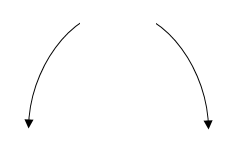
\includegraphics[width = 0.3\textwidth]{../Figures/polyEndBehaviorCopyBC.png}\item 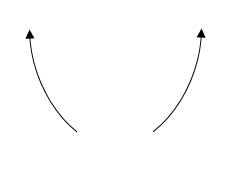
\includegraphics[width = 0.3\textwidth]{../Figures/polyEndBehaviorCopyCC.png}\item 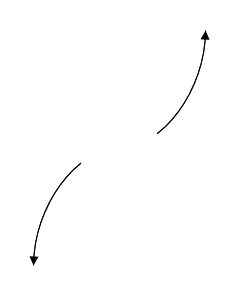
\includegraphics[width = 0.3\textwidth]{../Figures/polyEndBehaviorCopyDC.png}\end{multicols}\item None of the above.
\end{enumerate} }
\litem{
Which of the following equations \textit{could} be of the graph presented below?
\begin{center}
    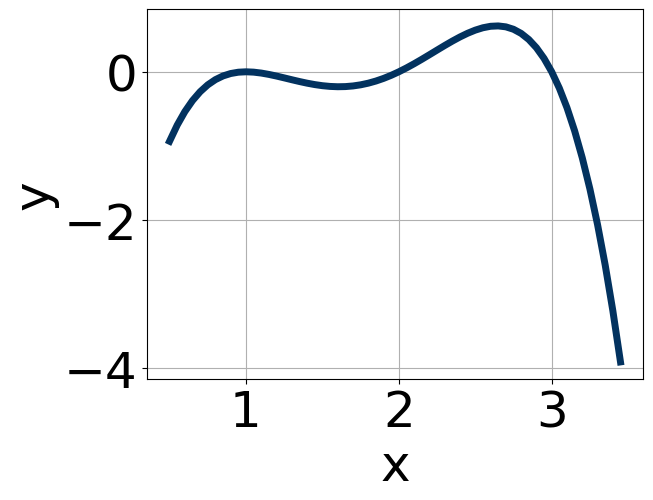
\includegraphics[width=0.5\textwidth]{../Figures/polyGraphToFunctionCopyC.png}
\end{center}
\begin{enumerate}[label=\Alph*.]
\item \( 10(x - 1)^{6} (x - 2)^{11} (x - 3)^{5} \)
\item \( -2(x - 1)^{4} (x - 2)^{5} (x - 3)^{11} \)
\item \( -10(x - 1)^{8} (x - 2)^{6} (x - 3)^{9} \)
\item \( -18(x - 1)^{7} (x - 2)^{10} (x - 3)^{7} \)
\item \( 19(x - 1)^{10} (x - 2)^{7} (x - 3)^{8} \)

\end{enumerate} }
\litem{
Describe the end behavior of the polynomial below.\[ f(x) = 6(x - 3)^{5}(x + 3)^{8}(x + 6)^{2}(x - 6)^{2} \]\begin{enumerate}[label=\Alph*.]
\begin{multicols}{2}\item 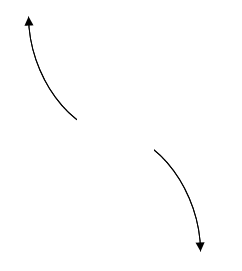
\includegraphics[width = 0.3\textwidth]{../Figures/polyEndBehaviorAC.png}\item 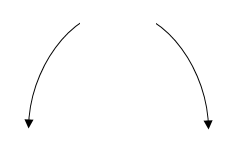
\includegraphics[width = 0.3\textwidth]{../Figures/polyEndBehaviorBC.png}\item 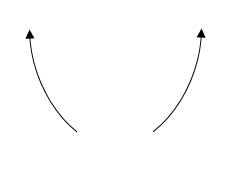
\includegraphics[width = 0.3\textwidth]{../Figures/polyEndBehaviorCC.png}\item 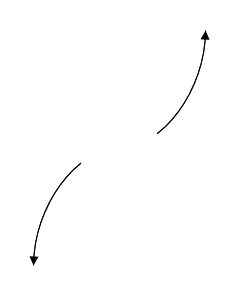
\includegraphics[width = 0.3\textwidth]{../Figures/polyEndBehaviorDC.png}\end{multicols}\item None of the above.
\end{enumerate} }
\end{enumerate}

\end{document}